
We consider a multiphase flow with no-mass transfer, i.e. $\textbf{u}_k=\textbf{u}_I$.
The interfaces have negligible weight and no interfacial viscosity. 

Then 

\subsection{Volume and Momentum conservation equations without mass transfer}

In this subsection we derive the mass and momentum conservation equation regardless of the shape of the particle as it will be reused in the following subsection. 
It is not necessary homogeneous. 
\subsubsection{The kinematic conservation equations}

To derive the volume conservation equations for the continuous pahse we set $f_{k} = 1$, $f_I = 0$ and  $\Phi_{k} = S_{k} =\Phi_{I} = S_{I} = 0$ for $k=1,2$. 
Applying this into \ref{eq:hybrid_avg_dt_chif} and using the conditional average definition from \ref{eq:1_avg} gives us,
\begin{equation}
    \pddt \phi_1
    + \nablabh \cdot (\phi_1 \oneavg{\textbf{u}})
    = 0.
    \label{eq:hybrid_avg_dt_chi}
\end{equation}
which is the transport equation of the continuous phase volume fraction, $\phi_1$,along the conditional phase velocity, $\oneavg{\textbf{u}}$. 

For the particle phase we first consider the volume of the particle, $v_\alpha = \int_{\Omega_\alpha} d\Omega$.
The volume occupied by the interface $v_{I\alpha}$, will not be considered since the thickness of the interfaces is not considered due to the sharp interface  hypothesis.
Instead,  we study the zeroth order moment of surface $s_{I\alpha} = \int_{\Sigma_\alpha} d\Sigma$. 
Injecting, $q_\alpha = 1$,$v_\alpha, s_{I\alpha}$ in \ref{eq:avg_dt_dq_alpha_tot} and making use of \ref{eq:p_avg} gives the number density, surface and volume particle-averaged equation, respectively,
\begin{align}
    \pddt n_p
    + \nablabh \cdot (\pnavg{\textbf{u}_\alpha})
    &= 
    0,
    \label{eq:hybrid_avg_dt_n}\\
    \pddt (\pnavg{s_{I\alpha}})
    + \nablabh \cdot (\pnavg{s_{I\alpha}\textbf{u}_\alpha})
    &= \pnavg{\dot{s}_{I\alpha}},
    \label{eq:hybrid_avg_dt_ds_alpha}\\
    \pddt (\pnavg{v_\alpha})
    + \nablabh \cdot (\pnavg{v_\alpha\textbf{u}_\alpha})
    &= 0,
    \label{eq:hybrid_avg_dt_dv_alpha}\\
\end{align}
It is important to understand that the RHS of both \ref{eq:hybrid_avg_dt_n} and \ref{eq:hybrid_avg_dt_dv_alpha} is zeroth due to the consideration of no mass transfer and no changes in topology such as coalesce ad break up.
However, in the surface equation we must consider a source term of the form $\dot{s}_{I\alpha} = \int_{\Sigma_\alpha} \textbf{u}_I \cdot \textbf{n}(\nablabh \cdot \textbf{n}) d\Sigma$ since the surface of a particle isn't constant under deformation \citep{morel2007surface}. 
Remark that the system of equation formed by \ref{eq:hybrid_avg_dt_n} to \ref{eq:hybrid_avg_dt_dv_alpha} share some similarities with the moment equations derived using Population Balance Equations (PBE)\citet{KAMP20011363,marchisio2013computational}.
The last equation is less common, it could also be considered as part of the PBE framework but as it will be presented in the next section it is rather usefull to predict the orientation of the particles. 

To reach a higher description of the dispersed phase we average \ref{eq:dt_M_alpha}, 
\begin{equation*}
    \pddt (\pnavg{\mathcal{M}^2_\alpha})
    + \nablab \cdot (
        \pnavg{\mathcal{M}^2_\alpha\textbf{u}_\alpha}
        )
    = 2\mathcal{S}_\alpha,
    \label{eq:hybrid_avg_dt_dM_alpha}
\end{equation*}
This equation will be useful to capture the particle shape or mass distribution of the particles. 

\subsubsection{The dynamic conservation equations}

Applying the averaged technics on \ref{eq:dt_p_alpha}, we easily derive the averaged momentum  equation of the phase $1$, namely,
\begin{equation}
    \pddt (\rho_1\phi_1\oneavg{\textbf{u}})
    +  \nablabh \cdot (\rho_1\phi_1\oneavg{\textbf{u}} \oneavg{\textbf{u}})
    = 
     \phi_1 \rho_1 \textbf{g}
    - \pnavg{\textbf{f}_\alpha}
    +  \nablab \cdot \left[
        \phi_1\oneavg{ \textbf{T}}
        + \mathbf{\Sigma}_P
    \right]
    \label{eq:hybrid_avg_dt_rhou}
\end{equation}
with $\textbf{f}_\alpha = \int_{\Sigma_\alpha} \mathbf{T}_1 \cdot \textbf{n}_2d\Sigma$ is the sum of the hydrodynamic forces applied on the particle. 
Following the method outlined in \citet{chu2016flux} we decompose the force into a large-scale stress contribution $\avg{\textbf{T}}$ and fluctuation stresses $\textbf{T}'_1$, which yields $\textbf{f}_\alpha = v_\alpha \nablab \cdot\avg{\textbf{T}}+ \int_{\Sigma_\alpha} \mathbf{T}'_1 \cdot \textbf{n}_2d\Sigma$ where we assumed $\nablab\cdot\avg{\textbf{T}}$ constant. 
\JL{surement pas que la "drag force". The sum of hydrodynamics forces on the particles. D'ailleurs je pense qu'il manque une etape. Ce terme ne peut pas etre interprete comme une force. Il faut lui soustraire la partie moyennee des contraintes. Cf bouquin de Jackson (section 2.2), Cours de Lhuillier equation (122) (qui fait quelque chose de legerement different) et papier de Zhang et Prosperretti (1997). Car sinon tu peux creer de la contrainte "juste" par effet d'inhomogeneite de fraction volumique. }
\tb{dans ce cas il faut retrancher aux premier moments hydro le gradient de pression, cela va devenir lourd en notation}
\tb{LIRE CHU ET Prosperetti et Quan et Prosperetti}
The tensor, $\mathbf{\Sigma}_P = \pnavg{\textbf{M}_\alpha} -  \rho_1\phi_1\oneavg{\textbf{u}'\textbf{u}'}$ is the particle contribution to the suspension stress.
\tb{ICI parler de l'expression du First moment Hydro en fonction de la phase interne}

Regarding the particle phase averaged equations, we consider at first the equation for the zeroth order of momentum, i.e. $\textbf{p}_\alpha = \int_{\Omega_\alpha} \rho_2 \textbf{u}_2 d\Omega$. 
By injecting $q_\alpha = \textbf{p}_\alpha$ in respectively, \ref{eq:avg_dt_dq_alpha_tot} and making use of the momentum decomposition when considering no mass transfer, $\textbf{p}_\alpha = \textbf{m}_\alpha \textbf{u}_\alpha$ from \ref{eq:momentum_definition}, \JL{Par ailleurs il manque un terme ou alors tu le neglige ?} \tb{pas de transfet de mass}
we obtain the following equation,

\begin{equation}
    \pddt (\pnavg{\rho_2 v_\alpha\textbf{u}_\alpha})
    + \nablabh \cdot(\pnavg{\rho_2 v_\alpha \textbf{u}_\alpha \textbf{u}_\alpha })
    = \pnavg{\rho_2 v_\alpha}\textbf{g}
    + \pnavg{\textbf{f}_\alpha}.
    \label{eq:hybrid_avg_dt_dp_alpha}\\
\end{equation}
First notice that in \ref{eq:hybrid_avg_dt_dp_alpha} has the same form as for solid spherical particle momentum conservation \citep{jackson1997locally} even-so we considered arbitrary particle shape and internal motion. 
Consequently, it is remarkable to observe that neither the surface tension nor the internal motion play a role in the linear momentum. 
Nevertheless, it is important to notice that due to the polydisperse nature of the flow we obtain mass weighted velocity terms $\pnavg{\rho_2 v_\alpha\textbf{u}_\alpha}$ and $\pnavg{\rho_2 v_\alpha\textbf{u}_\alpha\textbf{u}_\alpha}$. 
Therefore, this equation is not sufficient to describe the momentum of the particle phase, instead one have to solve for the size-weighted velocity moments corresponding to the Generalized Population Balance Equations (GPBE)  \citep{fox2023generalized}. 
In order to solve this equation for the averaged velocity, we suggest dividing the single particle momentum balance (\ref{eq:dt_q_alpha}), by the mass. 
Then, by applying the particle phase average on this acceleration balance gives, 
\begin{equation}
    \pddt (\pnavg{\textbf{u}_\alpha})
    + \nablabh \cdot(\pnavg{\textbf{u}_\alpha}\pnnavg{ \textbf{u}_\alpha })
    = 
    \pnavg{\frac{1}{v_\alpha\rho_2}\textbf{f}_\alpha}
    + n_p \textbf{g}
    - \nablabh \cdot(\pnavg{\textbf{u}'_\alpha \textbf{u}'_\alpha })
    \label{eq:hybrid_avg_dt_dp2_alpha}
\end{equation}
where $\pnavg{\textbf{u}'_\alpha \textbf{u}'_\alpha }$ and $\pnavg{(v_\alpha\rho_2)^{-1} \textbf{f}_\alpha }$, correspond respectively to the Reynolds stress tensor and the inverse mass weighted drag force term \citep{jackson1997locally}. 
Then we observe that the weighted velocity term vanish. 
Consequently, if we wish to describe poly disperse flows, two options are available. 
Either to solve for the size weighted velocity with the GPBE \citet{fox2023generalized,marchisio2013computational}.
Alternatively \ref{eq:hybrid_avg_dt_dp2_alpha} can be solved for the mean particle velocity with the weighted mass drag force term which is a function of the size-distribution.  
\JL{je ne comprends pas cette phrase} 
Therefore, it is more accurate to use \ref{eq:hybrid_avg_dt_dp2_alpha} than \ref{eq:hybrid_avg_dt_dp_alpha} in the case where we ignore the particle weighted average of the velocity. 
\tb{Some worlds about particle fluid particle stress and contact forces stress ? } \JL{pourquoi pas.}
\tb{finalement non le papier est deja trop log}



Then, the averaged conservation equation for $\mu_\alpha$, $\mathcal{S}_\alpha$ and $\mathcal{D}_\alpha$ can be obtained by taking the average of \ref{eq:dt_mu_alpha},\ref{eq:dt_S_alpha} and \ref{eq:dt_D_alpha} respectively.
It reads,
\begin{equation}
    \pddt (\pnavg{\mu_\alpha})
    + \nablabh\cdot (\pnavg{  \textbf{u}_\alpha \mu_\alpha})
    =  
    \pnavg{\textbf{t}_\alpha},
    \label{eq:hybrid_avg_dt_dmu_alpha}
\end{equation}
\begin{multline}    
    \pddt (\pnavg{\mathcal{S}_\alpha})
    + \nablabh\cdot (\pnavg{  \textbf{u}_\alpha \mathcal{S}_\alpha})
    =  \pnavg{\int_{\Omega_\alpha} \left(
        \rho_2\textbf{w}_2 \textbf{w}_2
        - \mathbf{T}_2
        \right) d\Omega}
        - \pnavg{\textbf{M}_\alpha^\sigma}
        + \pnavg{\textbf{S}_\alpha}.
    \label{eq:hybrid_avg_dt_dS_alpha}
\end{multline}
\begin{multline}
    \pddt (\pnavg{D_\alpha})
    + \nablabh\cdot (\pnavg{  \textbf{u}_\alpha D_\alpha})
    = \pnavg{\int_{\Omega_\alpha} \left(
        \rho_2 \textbf{w}_2 \cdot \textbf{w}_2
        - \mathbf{T}_2 : \textbf{I}
        \right) d\Omega}\\
        - 2\pnavg{\int_{\Sigma_\alpha} \sigma d\Sigma}
        + \pnavg{\int_{\Sigma_\alpha} \textbf{r}\cdot(\textbf{T}_1\cdot\textbf{n}_2) d\Sigma}
    \label{eq:hybrid_avg_dt_dD_alpha}
\end{multline}
\ref{eq:hybrid_avg_dt_dS_alpha} can also be seen as an equation for the averaged internal particle stress, by rearranging the terms yield, 
\begin{equation}    
    \pnnavg{\int_{\Omega_\alpha}\mathbf{T}_2d\Omega}
    = \pnnavg{ \int_{\Omega_\alpha} \rho_2 \textbf{w}_2 \textbf{w}_2d\Omega}
    - \pnnavg{ \ddt \mathcal{S}_\alpha}
    - \pnnavg{ \textbf{M}_\alpha^\sigma}
    + \pnnavg{  \textbf{S}_\alpha}
    \label{eq:T_definition}
\end{equation}
The determination of the internal particle stress is primordial in the study of Rheology.
As an example, for solid particles in Stokes regime $\int_{\Omega_\alpha} \rho_2 \textbf{w}_2 \textbf{w}_2d\Omega =  \ddt \mathcal{S}_\alpha = 0$ since no internal velocity are considered, and $\textbf{M}_\alpha^\sigma=0$ due to the solid nature of the particle. 
As a consequence this equation reduce to $\int_{\Omega_\alpha}\mathbf{T}_2d\Omega = \textbf{S}_\alpha$, which eventually leads us the computation of the Einstein viscosity. \tb{discuter w2w2 en stokes }
\JL{a detailler, meme si le calcul est naturel on ne peut pas juste le dire comme cela.}\tb{fait a peu près }
From \ref{eq:T_definition} we deduce that if one aim to compute the bulk stress at first order one must find closure for all terms of \ref{eq:T_definition}. 
By expressing each closure in terms of the bulk strain rate one could obtain a more general expression of the bulk viscosity. \tb{a develloper}



\subsection{First order equations for monodisperse axisymmetric particles with fore-aft symmetry}
\JL{Je pense qu'il faut etre honnete sur cette partie : on ne peut se contenter qu'une description phenomenlogique de ce qui se passe pour des particules non-spheriques. En particulier as tu lu la maniere dont sont fermes les equations dans le livre de Jackson et dans l'article de Zhang et Prosperreti pour des psheres en regime de Stokes ? c'est bien plus complique que de simplement donner la la loi de trainee sur une particule isolee. Cela fait nottament intervenir la loi de Faxen qui est tres complexe (pas de forme analytique) pour des particules non-spheriques. Je pense que cete partie doit discuter des particules solides allongees, mais aussi du cas des bulles de forme ellipsoidale applatie ("soucoupe volante"). Cela permet de couvrir deux cas limites. A discuter.}

To highlight the importance of the first order moments equations, we first take the example of mono-disperse solid axis symmetric particle suspension. 
In this case it is known that the orientation of the particles play a key role in the drag and hydrodynamic first moment models.
It is therefore primordial to fix a first order system of equation to capture this phenomenon.  
\begin{figure}[h!]
    \centering
    \hfill
    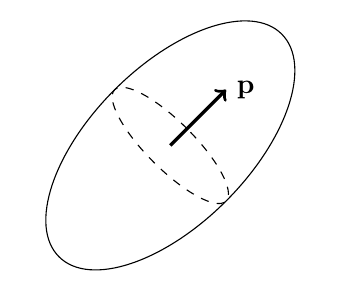
\begin{tikzpicture}[rotate=45]
        \draw(0,0) ellipse (2 cm and 1 cm);
        \draw[dashed](0,0) ellipse (0.3 cm and 1 cm);
        \draw[->,very thick](0,0) --++ (1,0)node[right]{$\textbf{p}$};
    \end{tikzpicture}
    \hfill
    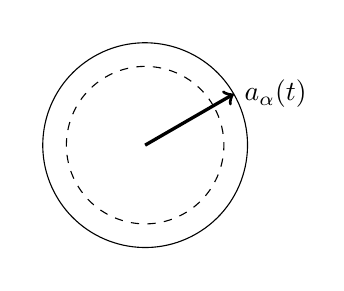
\begin{tikzpicture}[rotate=30]
        \draw(0,0) ellipse (1.3 cm and 1.3 cm);
        \draw[dashed](0,0) ellipse (1 cm and 1 cm);
        \draw[->,very thick](0,0) --++ (1.3,0)node[right]{$a_\alpha(t)$};
    \end{tikzpicture}
    \hfill
    \caption{Scheme of an axis symmetric particle with fore after symmetry and orientation normal vector \textbf{p}.}
    \label{fig:scheme2}
\end{figure}

\subsubsection*{Closures}
Initially we aim to solve the momentum equation for the fluid and particle phase \ref{eq:hybrid_avg_dt_rhou} and \ref{eq:hybrid_avg_dt_dp_alpha}. 
As previously mentioned these equations contain the following closures terms : $\oneavg{\textbf{T}}, \pnnavg{\textbf{f}_\alpha}, \pnnavg{\textbf{t}_\alpha}$ and $\pnnavg{\textbf{S}_\alpha}$ if we discard the fluctuation terms.
The closure for the averaged stress tensor appearing in \ref{eq:hybrid_avg_dt_rhou} can be express assuming solid unreformable motion inside the particles, with, \citep{jackson1997locally},

\subsubsection*{Bulk stress }
To derive the stress inside the bulk phase we follow , 
\begin{equation*}
    \avg{\textbf{T}}
    =  - \avg{p}\textbf{I}
    +2 \avg{\mu \textbf{E}}
\end{equation*}
where $p$ is the local pressure and $\textbf{E} = \sym{\nablab \textbf{u}}$ is the local strain rate tensor. 
It can be expressed as, 
\begin{equation*}
    \avg{\textbf{E}} 
    = \sum_k \avg{\chi_k\textbf{E}_k} 
    = \sym{\nablab \avg{\textbf{u}}} 
    + \sum_k \sym{\avg{\delta_I \textbf{n}_k \textbf{u}_k}}
\end{equation*}
If there is continuity of the normal velocity at the interface the second term on the RHS vanish. 
\begin{align*}
    \avg{\chi_k\textbf{E}_k} 
    &= \sym{\nablab \avg{\chi_k\textbf{u}_k}} 
    + \sym{\avg{\delta_I \textbf{n}_k \textbf{u}_k}}\\
    &= \sym{\nablab \avg{\chi_k\textbf{u}_k}} 
    - \sym{
        \avg{\delta_\alpha\int_{\Sigma_\alpha} \textbf{n}_k \textbf{u}_k d\Sigma}
        - \nablab\cdot\avg{\delta_\alpha\int_{\Sigma_\alpha} \textbf{r}\textbf{n}_k \textbf{u}_k d\Sigma}
        }
\end{align*}
then, 
\begin{equation*}
    \avg{\delta_\alpha\int_{\Sigma_\alpha} \textbf{n}_1 \textbf{u}_1 d\Sigma}
    = 
    \avg{
        \int_{\Omega_1} \nablab \textbf{u}_1 d\Omega
    }
\end{equation*}

This derivation is in agreement with \citet{zhang1997momentum}. 



Notice that the bulk velocity appearing in the above expression is in fact, $\avg{\textbf{u}} = \phi_1\oneavg{u} + \pnavg{\textbf{u}_\alpha} + \nablab\cdot (\pnavg{\mathcal{P}_\alpha})$.
Thus, the moment of momentum appear explicitly in the closure of the stress in agreement with \citet{zhang1997momentum}.  
Regarding the drag force, in  \citet{brenner1963resistance} they demonstrate that in low but finite inertia for an arbitrary shaped particle it could be expressed as,
\begin{equation}
    \textbf{f}_\alpha = 3 \pi \mu L \left[
        \textbf{R}_\alpha \cdot \textbf{U}
        + \frac{3}{16} Re  \left(
            3 \textbf{R}_\alpha 
            - \textbf{I} (\textbf{R}_\alpha : \textbf{e} \textbf{e})
        \right)
        \textbf{R}_\alpha\cdot  \textbf{U}
    \right]
\end{equation}
\JL{je pense pas que ce soit utile de citer Brenner \& Cox. On peut se limiter au regime de Stokes et juste dire que $\textbf{R}_\alpha$ depend de $\textbf{pp}$}
where $\textbf{U} = \oneavg{\textbf{u}}(\textbf{x}_\alpha)  - \textbf{u}_\alpha$ , $\textbf{e} = \textbf{U}/|\textbf{U}|$. 
and,  $\textbf{R}_\alpha$ is the resistance tensor in the laboratory frame. 
Besides, for axisymmetric particles with orientation vector \textbf{p} (sse \ref{fig:scheme2}) it can be shown that $\textbf{R}_\alpha = (R_{||} - R_\bot) \textbf{pp} + R_\bot \textbf{I}$, where $R_{||}$, $R_\bot$ are scalar coefficients \citep{guazzelli2011,kim2013microhydrodynamics}. 
Regarding the hydrodynamic torque applied on an asymmetric particle it can be expressed in Stokes regime as, 
\begin{equation}
    \textbf{t}_\alpha 
    = 
    \textbf{R}_{\omega T}\cdot \mathbf{\Omega}
     + \textbf{R}_{TU} \cdot \textbf{U} 
\end{equation}
where the first term represent the torque acting on the particle due to its translation,
with $R_T$ a correlation also function of the shape and $\textbf{U}$.
It must be noted that this relation remain partially true in low but finite inertial regime. 
Note that the correlation,  $R_T, R_{||} , R_{\bot}$ can be found in \citet{fintzi2023inertial} for cylindrical particles in dilute regime. 
And the second term represent the torque due to its rotation vector $\omega_\alpha$, where $\textbf{R}_{\omega T}$ is the resistance tensor linking rotation and torque \citet{pierson2021hydrodynamic} for inertial regime.  
Both $\textbf{R}_{\omega T}$ and $\textbf{R}_{TU}$ terms are function of the orientation of the particle \textbf{p}.
Closure for $\textbf{S}_\alpha$ can also be found but in the stokes regime only, 
indeed theoretical results are given in \citet[p 62]{kim2013microhydrodynamics}. Nevertheless, we do not provide them here as the expression is rather complicated. 
From the view of these closure terms we can see that in addition to the zeroth order terms, it is primordial to determine quantitatively the tensor $\textbf{pp}$, the rate of rotation $\omega_\alpha$ and the moment of momentum $\mathcal{P}_\alpha$. 

\subsubsection*{Dipole equations}
\JL{pourquoi dipole equations et pas first order moment equations ? l'expression dipole est utilise en mecanique des fluides mais pour des ecoulements potentiels generalement.}
Let consider a solid axis symmetric particle with fore after symmetric such that exposed in \ref{fig:scheme2}. 
Due to axis symmetric nature of the particle we can stipulate that, 
\begin{equation}
    \mathcal{M}_\alpha =  \textbf{pp} (M_\alpha^{||} - M_\alpha^\bot) 
    +  \textbf{I} M_\alpha^\bot
    \label{eq:M_definition}
\end{equation}
with $M_\alpha^{||}$, $M_\alpha^\bot$ being constant values related to the volume and shape of the particle. 
Besides, the velocity fields in inside each particle's domain can be deduced from solid body assumption, $\textbf{u}_2(\textbf{x}_\alpha + \textbf{r},t) = \textbf{u}_\alpha + \omega_\alpha \times \textbf{r}$ where $\omega_\alpha$ is the rotation vector of the particle $\alpha$.
By making use of this velocity decomposition it is easy to show that,
\begin{align}
    \mathcal{P}_\alpha
    &=  \omega_\alpha \times \left[
        \textbf{pp}(M_\alpha^{||} - M_\alpha^\bot) 
        + \textbf{I} M_\alpha^\bot
    \right]
    \label{eq:P_edfinition}\\
    2\mathcal{S}_\alpha
    &=  (M_\alpha^{||} - M_\alpha^\bot) \left(
        \omega_\alpha \times
        \textbf{pp}
        + \textbf{pp} \times \omega_\alpha
    \right)
    \label{eq:S_definition}\\
    \mu_\alpha / 
    &= \omega_\alpha \cdot \left[
        \textbf{pp} 
    (M_\alpha^{||}  - M_\alpha^{\bot} ) 
    - \textbf{I}(M_\alpha^{||} + M_\alpha^{\bot})
    \right]
    = \omega_\alpha \cdot\mathcal{I}_\alpha
    \label{eq:mu_definition}
\end{align}
Remark that  using the definition of $\mathcal{I}_\alpha$ yields a much simpler expression for $\mu_\alpha$. 

It is then straightforward to show that from \ref{eq:hybrid_avg_dt_dM_alpha},\ref{eq:S_definition} and \ref{eq:M_definition} we obtain the second order moment of volume conservation,
\begin{equation}
    \pddt (\pnavg{\textbf{pp}})
    + \nablab \cdot (
        \pnavg{\textbf{pp}\textbf{u}_\alpha}
        )
    = 
    \pnavg{\textbf{pp} \times \omega_\alpha}
    + \pnavg{\omega_\alpha \times \textbf{pp}} 
    % + \pnavg{\textbf{pp}' \times \omega_\alpha'}
    % +\pnavg{\omega_\alpha' \times \textbf{pp}'}
    \label{eq:hybrid_avg_dt_pp}
\end{equation}
In stokes flow we can find closure in the hypothesis of torque free particle, see \citet{kim2013microhydrodynamics}
\begin{equation}
    \omega_\alpha \times \textbf{p} 
    = -  \textbf{p} \times \omega_\alpha 
    = \avg{\Omega} \cdot \textbf{p} + \xi(\avg{\textbf{E}} \cdot \textbf{p} - \avg{\textbf{E}} \cdot \textbf{ppp})
    \label{eq:stokes_closure}
\end{equation}
Here $\avg{\textbf{E}}$ and $\avg{\Omega}$ are the symmetric and antisymmetric part of the velocity gradient. 
Injecting \ref{eq:stokes_closure} into \ref{eq:hybrid_avg_dt_pp} directly gives,
\begin{multline}
    \pddt (\pnavg{\textbf{pp}})
    + \nablab \cdot (
        \pnavg{\textbf{pp}\textbf{u}_\alpha}
        )
    = 
    \avg{\Omega} \cdot \pnavg{\textbf{pp}} 
    - \pnavg{\textbf{pp}} \cdot \avg{\Omega} \\
    + \beta\left[
        \avg{\textbf{E}} \cdot \pnavg{\textbf{pp}} 
        -\pnavg{\textbf{pp}} \cdot \avg{\textbf{E}} 
    - \avg{\textbf{E}} : \avg{\textbf{pppp}}
    \right]
    % \label{eq:hybrid_avg_dt_pp}
\end{multline}

In agreement with \citet{advani1987use} which found similar results except that they brought empirical expression for the fluctuation terms. \JL{je ne vois pas bien ou tu trouves cette equation dans le papier de Advani et Tucker ? D'ailleurs as tu lu Wang et Tucker 2008. Il est a mon avis plus explicite sur ce genre de chose.}

An equation for the rotation rate $\pnnavg{\omega_\alpha}$ can be obtained by, manipulating the angular momentum balance  \ref{eq:hybrid_avg_dt_dmu_alpha}, and using \ref{eq:mu_definition} and \ref{eq:hybrid_avg_dt_pp}, which gives,
\begin{multline}
    \left(
        \pnnavg{\textbf{pp}} 
        - \textbf{I}\frac{M_\alpha^{||} + M_\alpha^\bot}{M_\alpha^{||} - M_\alpha^\bot}
    \right)\left[
        \pddt (\pnavg{\omega_\alpha})
        + \nablab \cdot (
            \pnavg{\omega_\alpha}\pnnavg{\textbf{u}_\alpha}
            + \pnavg{\omega_\alpha'\textbf{u}_\alpha'})
        \right]\\
    +  \pnavg{\omega_\alpha}
    \cdot(\pnnavg{\omega_\alpha} 
    \times \pnnavg{\textbf{pp}})
    = \frac{\pnavg{\textbf{t}_\alpha}}{\rho_2}
    -\pnavg{\omega_\alpha' \cdot (\omega_\alpha \times \textbf{pp})'}
    +\pnavg{\omega_\alpha' \times \textbf{pp}}
    - \pnavg{\textbf{pp}'\dot{ \omega_\alpha}'}
\end{multline}
On the RHS we can observe that there is numerous closure fluctuation terms.  
\tb{FIND ref of this equations}\JL{as tu compare cette equation a celle de Zhang et Prosperreti 1997 ? }
\tb{they make spherical particle only so it is not interesting }
\subsubsection*{Stress equation}

Lastly, once we solved for $\pnnavg{\textbf{pp}}$ and $\pnavg{\omega_\alpha}$ we can deduce $\mathcal{S}_\alpha$ thanks to \ref{eq:S_definition}.
Afterward, we compute the integral of the undefined internal stress with \ref{eq:hybrid_avg_dt_dS_alpha}, which yield in our case, 
\begin{multline}
    \pnavg{\int_{\Omega_\alpha} 
        \mathbf{T}_2
    d\Omega}
    =  
      \pnavg{\textbf{S}_\alpha}
    - \rho_2\pnavg{\ddt \mathcal{S}_\alpha}\\
    - (M_\alpha^{||} - M_\alpha^\bot) \pnavg{
        (\omega_\alpha \times \textbf{p}) (\omega_\alpha \times \textbf{p}) } 
    -M_\alpha^\bot \pnavg{\textbf{I} \omega_\alpha^2 -\omega_\alpha\omega_\alpha }
    \label{eq:T2_definition}
\end{multline}
Then considering the particle nature it is possible to deduce its mean deformation from the stress integral, and validate or not the irreformability hypothesis made at start. 
It is also possible to compute the trace of the stress using \ref{eq:hybrid_avg_dt_dD_alpha}, yielding in this case, 
\begin{equation}
    \pnnavg{\int_{\Omega_\alpha} 
        \textbf{I}:\mathbf{T}_2
    d\Omega}
    =  
     (M_\alpha^{||} + M_\alpha^\bot) \pnnavg{
    \omega_\alpha^2} 
    - (M_\alpha^{||} - M_\alpha^\bot) \pnnavg{
    \omega_\alpha\omega_\alpha :  \textbf{pp}}
    + \pnnavg{\textbf{M}_\alpha} : \textbf{I}
\end{equation}
where we considered that the volume of the particle remained constant. 
This equation means that the rotational acceleration contribute to the isotropic particle pressure. 


In a pure rigorous manner the equivalent bulk stress of the suspension yield, 
\begin{equation*}
    \avg{\textbf{T}} = 
    \phi_1 \oneavg{\textbf{T}} 
    + \pnavg{\int_{\Omega_\alpha} \mathbf{T}_2 d\Omega}
    -\nablab\cdot \pnavg{\int_{\Omega_\alpha} \textbf{r}\mathbf{T}_2 d\Omega}
    + \ldots
\end{equation*}
Where the first and second terms on the RHS are given by \ref{eq:T_definition} and \ref{eq:T2_definition}, and the last one can be obtained with the third order moment of momentum equations. 
Anyhow, if we neglect this last term and if the solid motion hypothesis remain true we can determine the bulk stress using \ref{eq:T2_definition} which gives,
\begin{multline*}
    \avg{\textbf{T}} = 
    - \phi_1\oneavg{p}\textbf{I} 
    + \mu_1 \avg{\textbf{E}} 
    + \frac{1}{2}\frac{\pnavg{\textbf{S}_\alpha}}{\rho_2}
    - (M_\alpha^{||} - M_\alpha^\bot) \pnavg{\ddt \left(
        \omega_\alpha \times
        \textbf{pp}
        + \textbf{pp} \times \omega_\alpha
    \right)}\\
    - (M_\alpha^{||} - M_\alpha^\bot) \pnavg{
        (\omega_\alpha \times \textbf{p}) (\omega_\alpha \times \textbf{p}) } 
    -M_\alpha^\bot \pnavg{\textbf{I} \omega_\alpha^2 -\omega_\alpha\omega_\alpha }
\end{multline*}
Each term on the RHS can be for one part factorized by \textbf{I} yieldings the equivalent pressure of the suspension, and an other part by $\avg{\textbf{E}}$ yielding the equivalent viscosity. 



\tb{
\subsubsection*{Oblate bubbles}

As it has already mentioned the trace of the moment of momentum equation can be used to derive the Reyl
It is also possible to derive from the second moment of mass equation an equation for the mean aspect ratio $\pnnavg{\xi}$ of the particles.
Indeed, let's consider obalte particles, such as droplets or bubble, in this case the second moment of mass can be written, $\mathcal{M}_\alpha =  \textbf{pp} [M_\alpha^{||}(t) - M_\alpha^\bot(t)] +  \textbf{I} M_\alpha^\bot(t)$
\tb{As in tomiyama example they state that the shape of the particle is of particular importance here the moment of volume matter }


\subsubsection*{Spherical compressible bubbles}
As mentioned in the \ref{sec:Lagrangian} from teh trace of the moment of momentum equation we can recover the Rayleigh-Lamb-Plesset equation.
Thus, by using the averaged moment of momentum equation we can falll back on \citet{zhang1994ensemble} model.

\subsubsection*{Slightly deformable elastic particle}

Now let consider the momentum conservation of slightly deformable particles.
First, the velocity field inside the particles, is assumed linear and incompressible, such that $\textbf{u}(\textbf{y}_\alpha) = \textbf{u}_\alpha + \mathcal{L}_\alpha \cdot \textbf{r}$ where the second order tensor  $\mathcal{L}_\alpha= \textbf{e}_\alpha+ \boldsymbol{\omega}$, with $\textbf{e}$ and $\boldsymbol{\omega}$ are symmetric and skew-symmetric tensors, respectively.
It directly follows from the expression of the velocity : $\mathcal{P}_\alpha = \int_{\Omega_\alpha} \textbf{r}\textbf{u} d\Omega = \mathcal{L}_\alpha\cdot \mathcal{M}$

The constitutive equation of the stress, $\textbf{T}_2$, within the particle phase can be written such as $\textbf{T}_2 = \mathbb{C} : \textbf{e}_2$ for elastic materials, with $\mathbb{C}$ the fourth order stiffness tensor and $ \textbf{e}_2 = \frac{1}{2}\left(\nablab\textbf{u}_2+(\nablab\textbf{u}_2)^T\right)$ is the rate of strain symmetric tensor.
Making use of the internal velocity expression yield directly the relation, $\textbf{e}_2=\textbf{e}_\alpha\cdot$ in $\Omega_\alpha$.

We know that the deformation of the particles will not have an explicit impact on the linear conservation equations.
Thus, we will be interested into the first and second order momentum and mass conservation equations respectively.
Making use of the average of \ref{eq:dt_P_alpha} over every configuration of the flow, and using the previous properties yield an equation for the average stress tensor within the suspension, namely,
\begin{equation}
    \pnnavg{\int_{\Omega_\alpha}\textbf{T}_\alpha d\Omega}
    = n_p\mathbb{C} : \pnnavg{(\mathcal{L}_\alpha+ \mathcal{L}_\alpha^T) v_\alpha}
    % = - \mathcal{L}_\alpha\cdot \mathcal{L}_\alpha\cdot \mathcal{M}_\alpha
    % - \mathcal{M}_\alpha \cdot\ddt \mathcal{L}_\alpha
    % - \textbf{M}_\alpha
    \label{eq:hybrid_avg_dt_P_alpha}
\end{equation}
\begin{equation}
    \mathcal{M}_\alpha \cdot\ddt \mathcal{L}_\alpha
    = - \mathcal{L}_\alpha\cdot \mathcal{L}_\alpha\cdot \mathcal{M}_\alpha
    - \mathbb{C} : (\mathcal{L}_\alpha+ \mathcal{L}_\alpha^T) v_\alpha
    - \textbf{M}_\alpha
    \label{eq:hybrid_avg_dt_P_alpha}
\end{equation}
Besed on that kind of argument \citet{lhuillier1987phenomenology}
}


One last remark is in order. 
With \ref{eq:dt_S_alpha} it is possible to compute the integral of the undefined internal stress $\int_{\Omega_\alpha} 
\mathbf{T}_2
d\Omega$ within the particle phase.
But first,  for a prolate spheroid the $\textbf{S}_\alpha$ may be written with this quite lenthly expression : 
\begin{multline}
    \textbf{S}_\alpha 
    = \frac{20}{3}\pi \mu a^3 \left[
    \left(
        X^M \mathbf{p}^{(0)}+Y^M \mathbf{p}^{(1)}+Z^M \mathbf{p}^{(2)}
    \right) : \textbf{E}\right.\\ \left.
    + \frac{3}{5} Y^H ((\mathbf{\Omega} - \omega_\alpha) \times \textbf{pp} + \textbf{pp} \times (\mathbf{\Omega} - \omega_\alpha) )
    \right]
    \label{eq:S_def}
\end{multline}
where, $X^M$, $Y^M$,  $Z^M$ and $Y^H$ are scalar resistance function related to the shape of the particles, and the $\mathbf{p}^{(i)}$ are fourth order orientation tensor solely express in terms of $\textbf{p}$, all of which are given in \citet[p 62.]{kim2013microhydrodynamics}. 
theerfore, by rearranging the term for the integrated stress, \ref{eq:dt_S_alpha}, can be written for axissymmetric particles such as, 
\begin{multline}
    \pnavg{\int_{\Omega_\alpha} 
        \mathbf{T}_2
    d\Omega}
    =  
      \pnavg{\textbf{S}_\alpha}
    - (M_\alpha^{||} - M_\alpha^\bot)\pnavg{\ddt  \left(
        \omega_\alpha \times
        \textbf{pp}
        + \textbf{pp} \times \omega_\alpha
    \right) }\\
    - (M_\alpha^{||} - M_\alpha^\bot) \pnavg{
        (\omega_\alpha \times \textbf{p}) (\omega_\alpha \times \textbf{p}) } 
    -M_\alpha^\bot \pnavg{\textbf{I} \omega_\alpha^2 -\omega_\alpha\omega_\alpha }
\end{multline}
which is a constitutive expression of the stress. 
In stokes flow condition one may argue that all product of $\omega_\alpha$ and time derivative of $\omega$ are negligible, leavening with the stresslet. 